% ============================================================================
% Procedimiento de ensayo RE-TP-001 (TP1, entregable OE1)
% Base: esquema del procedimiento de Emisiones Radiadas provisto por la catedra.
% Un solo archivo .tex. Necesita en la misma carpeta: logo_fiuba.png,
% logo_materia.png, fig_esquema_general.png, fig_camara_anecoica.png y
% fig_camara_semianecoica.png.
% Compilar con pdfLaTeX (Overleaf: Menu > Compiler > pdfLaTeX).
% ============================================================================
\documentclass[11pt,a4paper]{article}

\usepackage[utf8]{inputenc}
\usepackage[T1]{fontenc}
\usepackage[spanish,es-tabla,es-nodecimaldot]{babel}
\usepackage[a4paper,margin=2.5cm,headheight=14pt]{geometry}
\usepackage{graphicx}
\usepackage{float}       % permite la opcion [H] en figuras y tablas
\usepackage{booktabs}
\usepackage{array}
\usepackage{longtable}
\usepackage{enumitem}
\usepackage{amsmath}
\usepackage{xcolor}
\usepackage{fancyhdr}
\usepackage{tikz}
\usetikzlibrary{babel}   % evita el choque entre TikZ y los atajos < > del español
\usepackage[hidelinks]{hyperref}

% ---------------------------------------------------------------- datos ----
\newcommand{\codigo}{RE-TP-001}
\newcommand{\version}{2.0 (borrador)}
\newcommand{\fecha}{19 de octubre de 2026}

% Texto que hay que completar o confirmar antes de usar el documento
\newcommand{\pendiente}[1]{\textcolor{red}{[#1]}}
% Casillero vacio para completar a mano
\newcommand{\casilla}{\rule{0pt}{4.2ex}}

\pagestyle{fancy}
\fancyhf{}
\lhead{\small \codigo{} -- Procedimiento de ensayo de Emisiones Radiadas (RE)}
\rhead{\small Versión \version}
\cfoot{\small \thepage}

\setlist{itemsep=2pt,topsep=4pt}

\begin{document}

% ============================================================== caratula ====
\begin{titlepage}
  \centering
  \vspace*{0.5cm}
  % logo de la facultad a la izquierda y logo de la materia a la derecha
  \begin{minipage}[c]{0.56\textwidth}
    \centering
    
\includegraphics[width=\textwidth]{logo_fiuba.png}
  \end{minipage}\hfill
  \begin{minipage}[c]{0.34\textwidth}
    \centering
    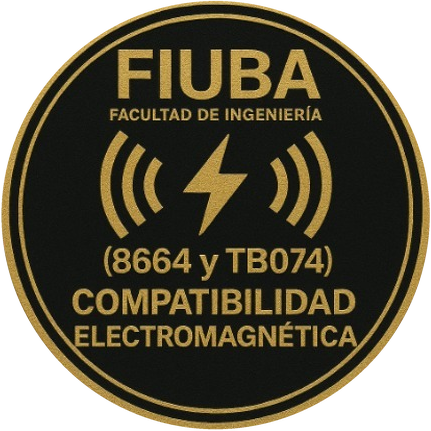
\includegraphics[width=\textwidth]{logo_materia.png}
  \end{minipage}\par
  \vspace{0.8cm}
  {\large Universidad de Buenos Aires -- Facultad de Ingeniería\par}
  {\large Compatibilidad Electromagnética (8664 y TB074)\par}
  {\large Trabajo Práctico N.\textsuperscript{o}~1 -- Entregable OE1\par}
  \vspace{1.6cm}
  {\Large \textsc{Procedimiento de ensayos}\par}
  \vspace{0.3cm}
  {\LARGE \bfseries Emisiones Radiadas (RE)\par}
  \vspace{0.6cm}
  {\Large Comb Generator basado en Software Defined Radio (SDR)\par}
  \vspace{0.8cm}
  {\large Código: \textbf{\codigo} \qquad Versión: \textbf{\version}\par}
  \vfill
  \begin{tabular}{ll}
    \toprule
    Autor               & Martín Ledesma \\
    Docentes            & Pablo Marino Belcaguy \\
                        & Walter Gustavo Fano \\
    Laboratorio         & CETEM, Florencio Varela \\
    Asistencia          & Federico Martinez (CETEM) \\
    Fecha               & \fecha \\
    \bottomrule
  \end{tabular}
  \vspace{1cm}
\end{titlepage}

% ====================================================== control de cambios ==
\section*{Control de versiones}
\begin{tabular}{@{}llp{8cm}@{}}
  \toprule
  Versión & Fecha & Cambios \\
  \midrule
  1.0 (borrador) & 5 de octubre de 2026 & Primera emisión. \\
  1.1 (borrador) & 12 de octubre de 2026 & Antena transmisora y ajustes para la primera medición en el CETEM. \\
  2.0 (borrador) & \fecha & Entregable OE1: la SDR como EUT en su papel de calibrador, límites de CISPR~11, tres alturas de antena, incertidumbre de medición y lo aprendido en la medición del 13-10-2026. El manejo del software y la calibración de la fuente pasan al manual de la SDR (OE2). \\
  \bottomrule
\end{tabular}

\section*{Participantes}
\begin{tabular}{@{}lp{10cm}@{}}
  \toprule
  Persona & Función en el ensayo \\
  \midrule
  Martín Ledesma        & Opera la SDR y el software y registra los resultados. \\
  Federico Martinez     & Opera la cámara, el mástil, la mesa y el receptor del CETEM. \\
  Pablo Marino Belcaguy & Docente, revisión del procedimiento. \\
  Walter Gustavo Fano   & Docente, revisión del procedimiento. \\
  \bottomrule
\end{tabular}

\tableofcontents
\newpage

% ============================================================================
\section*{Procedimiento de ensayos Emisiones Radiadas (RE)}

Para evaluar las emisiones radiadas de un Comb Generator basado en SDR bajo normativas estándar de compatibilidad electromagnética (CISPR 11 / ANSI C63.4), se estructura un Procedimiento de Ensayo de Emisiones Radiadas (\emph{Radiated Emissions Test Procedure}) estándar de laboratorio.

\begin{figure}[H]
  \centering
  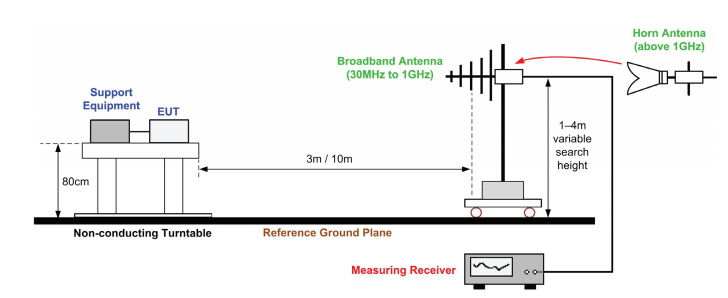
\includegraphics[width=0.85\textwidth]{fig_esquema_general.png}
  \caption{Disposición general de un ensayo de emisiones radiadas.}
\end{figure}

\begin{figure}[H]
  \centering
  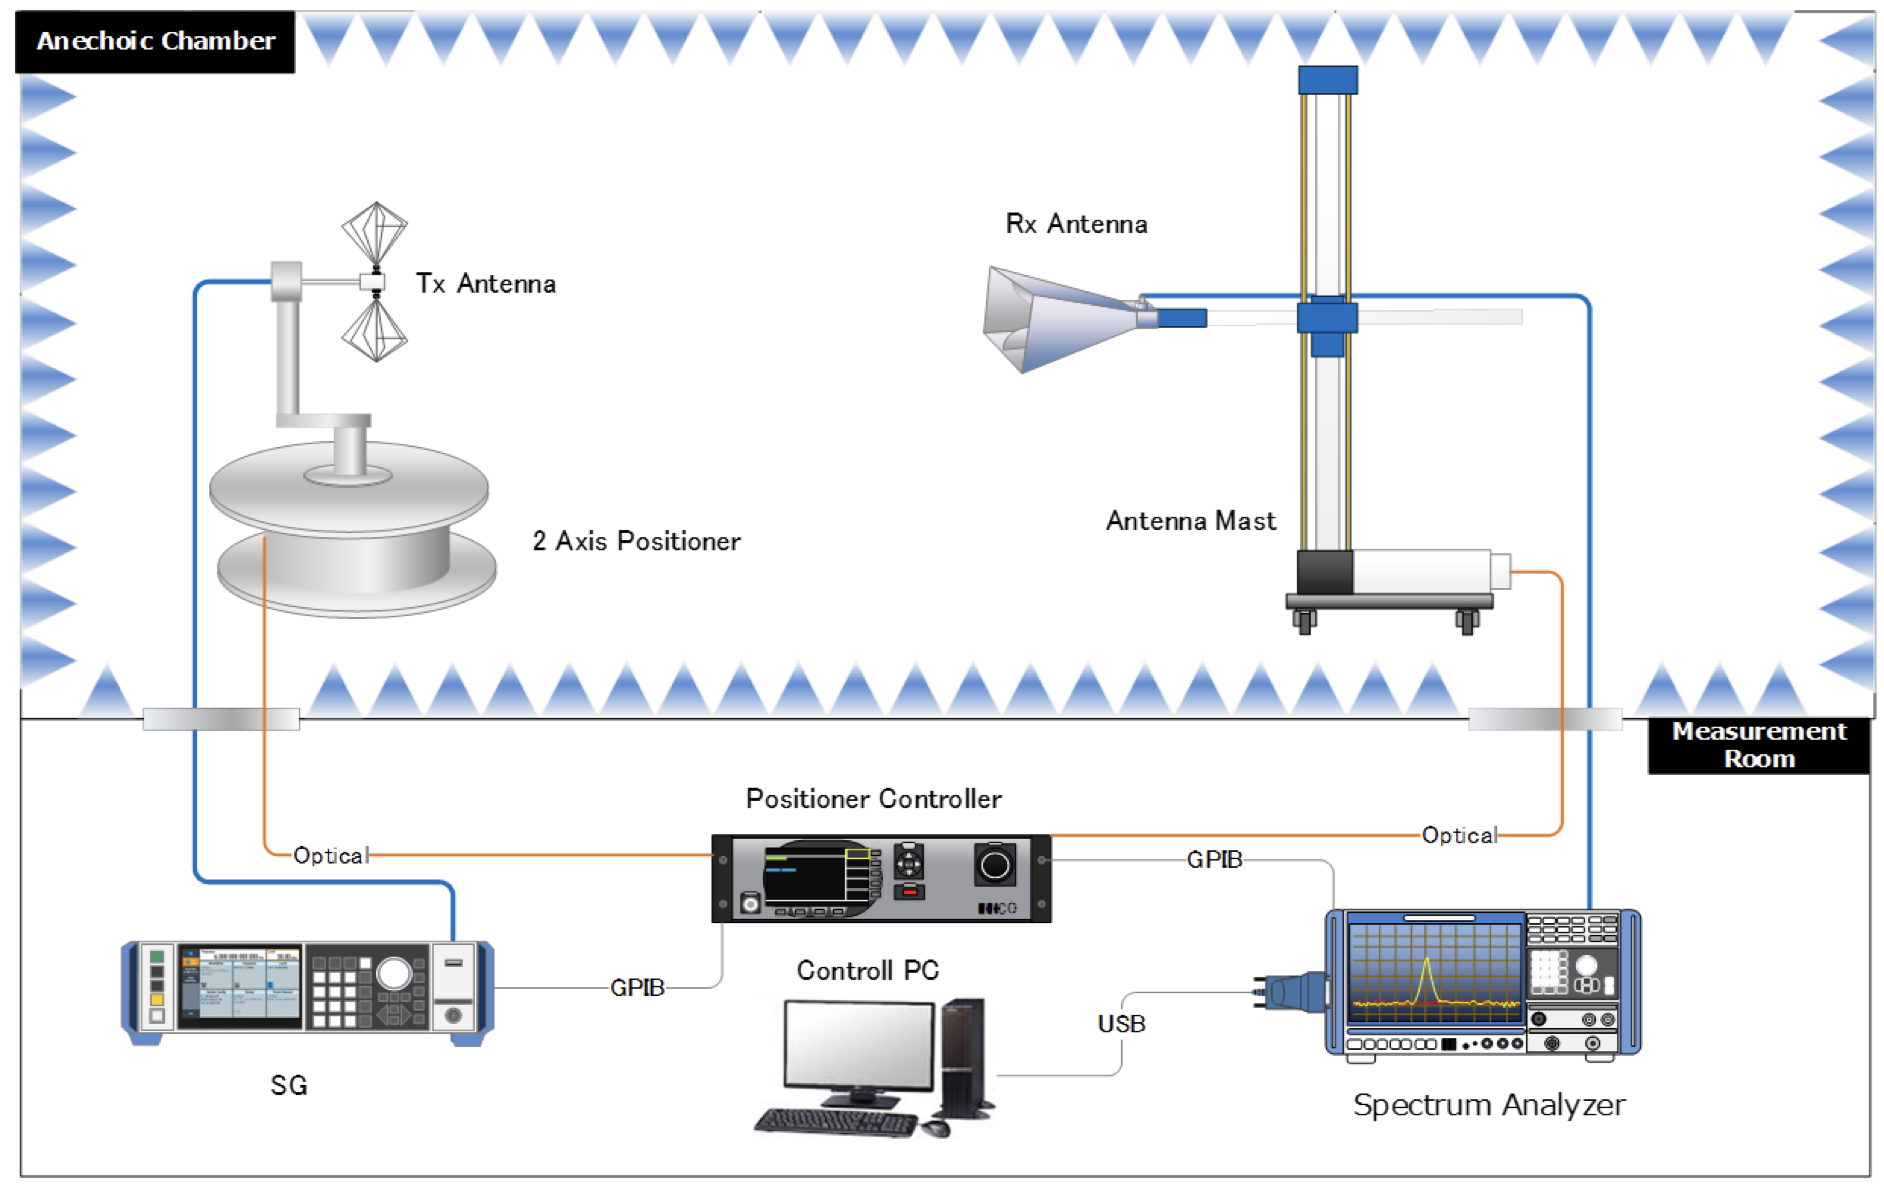
\includegraphics[width=0.85\textwidth]{fig_camara_anecoica.png}
  \caption{Cámara y sala de medición.}
\end{figure}

\newpage
\begin{center}
  {\large\bfseries PROCEDIMIENTO DE ENSAYO DE EMISIONES RADIADAS (\codigo)}
\end{center}

% ============================================================================
\section{Objeto y alcance}

Este documento define los pasos para la caracterización y verificación de emisiones radiadas en el dominio de la frecuencia del equipo \textbf{EUT/DUT: Comb Generator basado en Software Defined Radio (SDR)}.

La SDR es el EUT en su papel de calibrador: lo que se mide es el peine que emite, que sirve de referencia para la cadena de medición. También se registran sus emisiones propias, en pausa y emitiendo sin antena, porque son el fondo contra el que se leen las líneas del peine.

\begin{itemize}
  \item \textbf{Normas de referencia aplicables:} CISPR 16-1-1, CISPR 16-2-3, CISPR 16-4-2, CISPR 11 (grupo 1, clase B), ANSI C63.4.
  \item \textbf{Rango de frecuencia:} 30~MHz a 1~GHz, ampliable hasta 6~GHz según la frecuencia máxima que transmita la SDR. El peine de esta versión cubre de 60 a 980~MHz.
\end{itemize}

\paragraph{Finalidad.} El Comb Generator se usa como \emph{fuente de referencia} para verificar la cadena de medición de emisiones radiadas del laboratorio y controlar su continuidad en el tiempo. Emite 24 líneas entre 60 y 980~MHz, una cada 40~MHz, calibradas por conducción a un nivel fijo: 0~dBm~$\pm$~1~dB en esta versión \pendiente{revisar al bajar el nivel del peine}. La primera medición en la cámara establece la \emph{curva de referencia}, mientras que las mediciones posteriores se comparan contra ella. Si el mismo peine, montado de la misma forma, se recibe distinto, lo que cambió es la cadena de medición.

\begin{itemize}
  \item \textbf{Qué verifica:} la cadena completa: cámara, antena de medición, cables y receptor.
  \item \textbf{Límites normativos:} el peine es un emisor intencional, por lo que el resultado no se evalúa como conformidad. Los límites de CISPR~11 (tabla~\ref{tab:limites}) se grafican junto a las líneas y se informa el margen de cada una, como referencia.
  \item \textbf{Validez:} los resultados valen para el montaje descrito en la sección~\ref{sec:montaje}. Cambiar la antena transmisora, su posición, las alturas de la antena de medición o el recorrido del cable USB obliga a tomar una curva de referencia nueva.
\end{itemize}

\begin{table}[H]
  \centering
  \begin{tabular}{@{}lcc@{}}
    \toprule
    Banda & A 3~m (dB$\mu$V/m) & A 10~m (dB$\mu$V/m) \\
    \midrule
    30 a 230~MHz   & 40 & 30 \\
    230 a 1000~MHz & 47 & 37 \\
    \bottomrule
  \end{tabular}
  \caption{Límites de CISPR~11 para equipos del grupo~1, clase~B, en cámara semianecoica (cuasi-pico). En 230~MHz vale el límite más estricto.}
  \label{tab:limites}
\end{table}

% ============================================================================
\section{Equipamiento y medios de ensayo}

\begin{itemize}
  \item \textbf{Entorno:} Cámara Semianecoica (SAC) calibrada a 3 metros (o 10 metros).
  \item \textbf{Receptor EMI:} Cumplimiento con CISPR 16-1-1. En el CETEM: R\&S ESR-7.
  \item \textbf{Modo:} Detector Quasi-Peak y Peak, RBW 120~kHz de 30~MHz a 1~GHz; RBW 1~MHz por encima de 1~GHz. En este procedimiento se usa el detector Peak con MAX HOLD (ver sección~\ref{sec:pasos}).
  \item \textbf{Antenas de Medición:}
        \begin{itemize}
          \item Biconical (30~MHz -- 300~MHz).
          \item Log-Periodic / Bilog Hybrid (30~MHz -- 1~GHz). En el CETEM: antena bilog \pendiente{modelo}, con su factor de antena y la pérdida del cable cargados en el receptor como transductor.
          \item Horn.
          \item Mástil de antena motorizado (1~m a 4~m de altura, o hasta la altura máxima de la cámara).
        \end{itemize}
  \item \textbf{Mesa Giratoria (Turntable):} no metálica, a 0,8~m de altura respecto al plano de masa.
  \item \textbf{Cables y atenuadores:} de baja pérdida, con la pérdida medida. Para la SDR, cable USB 3.0 de alta velocidad y larga distancia.
  \item \textbf{SDR} con sus accesorios para poder utilizarla, incluyendo la antena, e incluyendo shield que evite interferencias de la misma SDR.
        \begin{itemize}
          \item bladeRF 2.0 micro xA9, número de serie \texttt{321e0fa5875945d99b11070bb0a76d31}.
          \item Antena transmisora: telescópica de 30~cm, totalmente extendida (hasta el tope) y vertical, en el conector TX1. Siempre la misma y siempre extendida igual.
          \item Carga de 50~$\Omega$ para el conector TX1, para medir la emisión de la placa sin antena.
          \item Caja metálica: \pendiente{falta definir}.
          \item Ferrita para el cable USB.
        \end{itemize}
  \item \textbf{Software asociado a la SDR:} GNU Radio 3.10, con:
        \begin{itemize}
          \item el flujo \texttt{exp26\_a9\_peine\_radiado\_desde60.grc};
          \item el archivo de calibración \texttt{calibracion\_peine\_desde60.txt}.
        \end{itemize}
        Su manejo y la calibración de la fuente se describen en el \emph{Manual y procedimiento funcional de la SDR} (OE2).
  \item \textbf{Computadora} para manejar la SDR desde afuera, conectada por el cable USB instalado entre la sala de control y la cámara. \pendiente{Confirmar con el CETEM que ese cable sea USB~3: el 13-10-2026 la notebook quedó dentro de la cámara, sobre la mesa, con un cable corto.}
  \item Analizador de espectro portátil (tinySA Ultra) y cable coaxial, para verificar la fuente por conducción antes de entrar a la cámara.
\end{itemize}

\paragraph{Referencias.}
\begin{itemize}
  \item YRS03, Eurofins York, Comb Generator: referencia comercial del tipo de fuente.
  \item bladeRF 2.0 micro, Nuand. Potencia de salida CW: +8~dBm.
\end{itemize}

\paragraph{Precauciones.}
\begin{itemize}
  \item Emitir solo dentro de la cámara: el peine cae sobre bandas de radiodifusión, aeronáutica y telefonía. Fuera de la cámara la SDR se conecta únicamente por cable a un analizador.
  \item Analizador portátil: atenuación interna fija en 30~dB antes de subir la ganancia de la SDR a 55 o 65~dB.
  \item Nunca conectar la salida TX de la SDR a su entrada RX.
  \item El software arranca en \textsc{pausa}. Destildarla solo con el montaje terminado y la cámara cerrada.
  \item Si el programa se cierra solo o muestra errores de USB, desenchufar la SDR, esperar un minuto y volver a enchufarla.
\end{itemize}

% ============================================================================
\section{Configuración del DUT}\label{sec:montaje}

\begin{figure}[H]
  \centering
  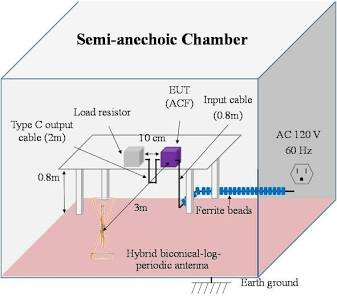
\includegraphics[width=0.55\textwidth]{fig_camara_semianecoica.png}
  \caption{Montaje de un equipo de mesa en la cámara semianecoica.}
\end{figure}

Colocar el SDR (Comb Generator) sobre la mesa giratoria no conductiva a $0{,}8$~m sobre el plano de tierra reflejante.

Cables de alimentación / control: si el SDR requiere conexión USB/Power a una PC host, la PC debe ubicarse fuera de la cámara o blindarse debidamente. Si se usan cables dentro de la cámara, colocar un filtro/ferrita según marca la norma ANSI C63.4 para evitar que los cables actúen como antenas no deseadas.

Configurar el script del SDR para emitir el patrón de peine deseado. En este procedimiento el patrón es el descrito en la sección~\ref{sec:sdr}: 24 líneas de 60 a 980~MHz, una por vez.

\paragraph{Geometría: mesa fija y tres alturas.} La medición de rutina se hace sin girar la mesa y con la antena de medición en tres alturas fijas, en las dos polarizaciones. Con tres alturas ninguna línea depende de una sola posición, que podría caer en un mínimo por el reflejo en el piso: el 13-10-2026, al cambiar la altura, cada línea varió una mediana de 7,9~dB. Las alturas se adaptan a cada cámara: por defecto 1, 2 y 3~m; en una cámara con mástil de 2~m, 1~m, 1,5~m y 2~m. Una vez elegidas, son siempre las mismas en ese laboratorio. El ángulo de la mesa se elige una sola vez, en el barrido preliminar (paso~\ref{paso:prescan}).

\begin{figure}[H]
  \centering
  \begin{tikzpicture}[font=\small,>=latex]
    \draw[line width=1.2pt] (-1,0) -- (11,0);
    \node[below] at (5,0) {Plano de tierra reflectante};
    \draw (0.2,0) -- (0.2,1.6) (1.8,0) -- (1.8,1.6);
    \draw[line width=1pt] (0,1.6) -- (2,1.6);
    \draw[fill=gray!25] (0.7,1.6) rectangle (1.3,1.9);
    \draw[line width=0.8pt] (1.0,1.9) -- (1.0,2.6);
    \node[above] at (1.0,2.6) {SDR + antena};
    \draw[<->] (-0.4,0) -- (-0.4,1.6) node[midway,left] {0,8 m};
    \draw[dashed] (0.7,1.7) -- (0.45,1.7) -- (0.45,0.05) -- (-1,0.05);
    \node[left] at (-1,0.05) {USB a la PC};
    \draw[line width=1pt] (9,0) -- (9,3.4);
    \draw[line width=0.8pt] (8.2,3.0) -- (9,3.0);
    \foreach \x/\h in {8.25/0.45,8.45/0.38,8.65/0.30,8.85/0.22}
      \draw (\x,3.0-\h) -- (\x,3.0+\h);
    \node[above] at (8.9,3.5) {Antena de medición};
    \draw[<->] (9.5,0) -- (9.5,3.0) node[midway,right] {$h_1$, $h_2$, $h_3$};
    \draw[<->] (1.0,0.6) -- (9,0.6) node[midway,above] {3 m};
    \draw (9,0.05) -- (11,0.05);
    \node[right] at (11,0.05) {al receptor};
  \end{tikzpicture}
  \caption{Montaje usado en este procedimiento. La PC y el receptor quedan fuera de la cámara.}
\end{figure}

\begin{enumerate}
  \item Colocar la SDR en el centro de la mesa, con la antena transmisora vertical.
  \item Bajar el cable USB recto hasta el piso y llevarlo al pasamuros siempre por el mismo recorrido. Colocar la ferrita junto a la SDR.
  \item Ubicar la antena de medición a 3~m, en la primera de las tres alturas.
  \item Fotografiar el montaje desde dos lados. Las fotos forman parte de la curva de referencia: en cada medición posterior el montaje se arma igual que en las fotos.
\end{enumerate}

\begin{table}[H]
  \centering
  \begin{tabular}{@{}lll@{}}
    \toprule
    Parámetro & Valor por defecto & Usado el 13-10-2026 \\
    \midrule
    Distancia de medición             & 3~m          & 3~m \pendiente{confirmar} \\
    Altura de la mesa                 & 0,8~m        & \pendiente{confirmar} \\
    Ángulo de la mesa                 & 0\textdegree & 0\textdegree \\
    Alturas de la antena de medición  & 1, 2 y 3~m   & 1, 2 y 3~m \\
    Polarizaciones                    & H y V        & V \\
    Orientación de la SDR             & conector TX hacia la antena & \pendiente{completar} \\
    \bottomrule
  \end{tabular}
  \caption{Geometría. En la primera medición de cada laboratorio se fijan los valores definitivos.}
  \label{tab:geometria}
\end{table}

% ============================================================================
\section{Procedimiento paso a paso}\label{sec:pasos}

Antes de entrar a la cámara se verifica la fuente por conducción (anexo~\ref{anexo:previa}).

\begin{enumerate}[label=\textbf{\arabic*.},leftmargin=*,itemsep=8pt]

  \item\label{paso:receptor} \textbf{Configuración del Receptor según CISPR 16-1-1:} ajustes en el analizador de espectro / receptor EMI.
        \begin{enumerate}[label=\arabic*.]
          \item Frecuencia de inicio 30~MHz y de parada 1~GHz.
          \item RBW de 120~kHz y VBW de 300~kHz.
          \item Detector Peak con MAX HOLD.
          \item Transductor cargado: factor de antena y pérdida del cable. Anotar cuál.
          \item Atenuador interno y preamplificador: elegirlos una vez y no cambiarlos en toda la campaña, porque el piso de ruido cambia con ellos (el 13-10-2026, al pasar de 10 a 20~dB de atenuación, el piso subió 10~dB). Anotarlos.
          \item Tiempo de barrido menor que la mitad del tiempo que cada línea está encendida (sección~\ref{sec:sdr}). \pendiente{Definir con el CETEM el modo de barrido: según el encabezado de las trazas del 13-10-2026, se usó un paso de 30~kHz y 50~ms por punto, que daría unos 27~min por barrido.}
        \end{enumerate}

  \item \textbf{Medición del Ruido de Fondo (Ambient Noise):} Verificación previa del entorno.

        Desactivar o apagar el SDR.

        Ejecutar un barrido rápido en detector Peak desde 30~MHz hasta la máxima frecuencia de interés. Verificar que el nivel de ruido ambiental esté al menos \textbf{6~dB por debajo} de los límites normativos aplicables (tabla~\ref{tab:limites}). Se verifica entonces que el ruido quede al menos 10~dB por debajo del nivel con que después se reciben las líneas del peine. Guardar la traza.

  \item\label{paso:prescan} \textbf{Barrido Preliminar (Prescan):} Identificación de armónicos del Comb Generator.
        \begin{enumerate}[label=\arabic*.]
          \item Encender la SDR sin modo COMB, en modo stand by, y se mide todo. En el software: ejecutar el flujo y dejarlo en \textsc{pausa}. Tomar una traza en MAX HOLD durante un minuto y guardarla: muestra lo que emite la placa por sí sola (su reloj y el USB).
          \item Cambiar la antena transmisora por la carga de 50~$\Omega$, destildar \textsc{pausa} y guardar una pasada completa: muestra lo que irradia la placa sin antena. Volver a tildar \textsc{pausa} y colocar la antena.
          \item Poner la SDR en modo de generación de ``Comb'': calibración importada, ganancia 65~dB, silencio entre saltos activado, destildar \textsc{pausa}.
          \item Configurar el receptor EMI en \textbf{Max Hold (Peak)} con un barrido rápido.
          \item Girar la mesa 360\textdegree{} continuamente y variar la altura de la antena entre 1~m y 4~m (o hasta la altura máxima de la cámara) en ambas polarizaciones (Horizontal y Vertical) para mapear los picos principales del peine de frecuencias.
        \end{enumerate}
        El punto 1 se repite en cada medición; los puntos 2 y 5, \textbf{solo la primera vez}. El resultado del punto 5 es el ángulo de la mesa, junto con la confirmación de que en ninguna de las tres alturas las 24 líneas quedan en un mínimo. Anotarlo en la tabla~\ref{tab:geometria}. Si no hay tiempo, usar los valores por defecto.

  \item \textbf{Medición Final:} con la geometría de la tabla~\ref{tab:geometria}.
        \begin{enumerate}[label=\arabic*.]
          \item Mesa en el ángulo elegido; antena de medición en la primera altura, polarización horizontal.
          \item Verificar que el silencio entre saltos esté activado y que el 3.\textsuperscript{er} LED de la SDR quede encendido fijo.
          \item Reiniciar MAX HOLD. Anotar el número de paso que muestra la ventana del software y esperar a que vuelva a ese mismo número: es una pasada completa (4~min~48~s con silencio).
          \item Comprobar que se ven líneas cada 40~MHz (60, 100, 140, \dots, 980~MHz) y que cada una supera en al menos 10~dB a las fugas de portadora y al piso de ruido.
          \item Guardar la traza (imagen y datos).
          \item Repetir los puntos 3 a 5 en las otras dos alturas y después en polarización vertical: seis trazas en total, unos 30~minutos.
          \item Leer el nivel de las 24 líneas en cada traza y completar las tablas de la sección~\ref{sec:registro}.
        \end{enumerate}

        \emph{Maximización (cumplimiento con CISPR / ANSI).} El método normativo, para cada armónico o frecuencia crítica identificada en el Prescan, es:
        \begin{enumerate}[label=\arabic*.]
          \item Posicionar la mesa en el ángulo $\theta$ donde la emisión sea máxima.
          \item Elevar/bajar el mástil de antena entre 1~m y 4~m para encontrar el pico por interferencia con el suelo.
          \item Cambiar la polarización de la antena (Horiz / Vert) para encontrar el nivel máximo de $E_{radiado}$.
          \item Aplicar el detector \textbf{Quasi-Peak (QP)} con tiempo de integración de 1~segundo por punto.
        \end{enumerate}
        En esta versión no se aplica en la medición de rutina, por dos motivos: para controlar continuidad interesa repetir siempre la misma geometría, y el generador emite una línea por vez (6~s cada 12~s), lo que no permite detenerse en una línea para maximizarla ni medirla en cuasi-pico. Queda como ampliación.

  \item \textbf{Repetibilidad (solo la primera vez).} Desmontar todo, volver a montar siguiendo las fotos y repetir la medición final. La diferencia entre las dos es la repetibilidad del montaje, y sirve para confirmar o ajustar las tolerancias de la sección~\ref{sec:criterio}.

  \item \textbf{Cálculo de Campo Eléctrico Real:} El valor final de campo eléctrico medido $E_{dB\mu V/m}$ se calcula como:
        \begin{equation}
          E_{dB\mu V/m} = V_{receptor}\,(dB\mu V) + AF\,(dB/m)
            + L_{cable}\,(dB) - G_{amp}\,(dB)
        \end{equation}

        \textbf{Importante:}
        \begin{itemize}
          \item $AF$ es el factor de antena, dado por la calibración del fabricante. Tiene que estar cargado en el receptor de EMI.
          \item $L_{cable}$, las pérdidas del cable, tienen que estar medidas: introducen un error sistemático en la medición. Conviene que sean mínimas, menores a 1~dB, para que influyan muy poco.
          \item $G_{amp}$ es la ganancia del preamplificador, si se usa. Verificar si está encendido o apagado y anotarlo.
        \end{itemize}

        Para controlar continuidad alcanza con comparar la lectura del receptor, siempre que $AF$, $L_{cable}$ y $G_{amp}$ sean los mismos que en la curva de referencia. Un cambio en cualquiera de ellos es justamente lo que este procedimiento detecta; por eso se anotan en el registro.
\end{enumerate}

\paragraph{Cierre.} Tildar \textsc{pausa}, cerrar el programa y desenchufar la SDR. Guardar capturas, fotos y el registro en una carpeta con la fecha.

% ============================================================================
\section{Registro y reporte}\label{sec:registro}

\begin{itemize}
  \item Gráfica del espectro completo (30~MHz -- 1~GHz) con los límites de CISPR~11 grupo~1 clase~B (tabla~\ref{tab:limites}) y la curva de referencia del peine.
  \item Tabla de picos con: Frecuencia, Nivel medido, Límite, Margen ($dB$), Referencia, Diferencia ($dB$), Ángulo de mesa (\textdegree), Altura de antena ($m$) y Polarización ($H/V$). El ángulo de la mesa es el mismo para todas las líneas y se anota una sola vez.
  \item Trazas del ruido de fondo y de la emisión propia de la SDR (en pausa y sin antena), fotos del montaje y captura de la verificación previa por conducción.
\end{itemize}

\subsection{Criterio de aceptación}\label{sec:criterio}

Para cada línea, cada altura y cada polarización se calcula la diferencia entre el nivel medido y el de la curva de referencia.

\begin{table}[H]
  \centering
  \begin{tabular}{@{}ll@{}}
    \toprule
    Diferencia con la referencia & Resultado \\
    \midrule
    Hasta $\pm$3~dB          & Conforme \\
    Entre $\pm$3 y $\pm$6~dB & Revisar el montaje contra las fotos y repetir \\
    Más de $\pm$6~dB         & No conforme: investigar la cadena de medición \\
    \bottomrule
  \end{tabular}
  \caption{Criterio de continuidad. Valores iniciales, a confirmar con el paso de repetibilidad.}
\end{table}

Los 3~dB resultan de sumar la tolerancia de la fuente ($\pm$1~dB) y la repetibilidad esperada al volver a montar. Las líneas que no superen por 10~dB al ruido de fondo y a la emisión propia de la SDR se marcan y no se usan para el criterio. El margen respecto del límite se informa, pero no entra en el criterio.

Si varias líneas contiguas se apartan en el mismo sentido, conviene sospechar de un elemento con respuesta en frecuencia (antena, cable, preamplificador). Si todas se apartan por igual, de una ganancia o una atenuación. Si la verificación previa por conducción no dio 0~dBm~$\pm$~1~dB, el problema está en la fuente y no en la cadena.

\subsection{Planilla}

\begin{tabular}{@{}p{6.3cm}p{8.5cm}@{}}
  \toprule
  Fecha y hora                         & \casilla \\
  Operadores                           & \casilla \\
  ¿Curva de referencia o verificación? & \casilla \\
  Receptor, antena y cables usados     & \casilla \\
  Transductor cargado en el receptor   & \casilla \\
  Atenuador interno del receptor (dB)  & \casilla \\
  Preamplificador (sí/no, ganancia)    & \casilla \\
  Ángulo de mesa y alturas de antena   & \casilla \\
  Silencio entre saltos activado (sí/no) & \casilla \\
  PC dentro o fuera de la cámara       & \casilla \\
  Fecha de la calibración de la fuente & \casilla \\
  Verificación previa: rango de las 24 líneas por conducción (dBm) & \casilla \\
  Tiempo de barrido del receptor       & \casilla \\
  Archivos guardados                   & \casilla \\
  \bottomrule
\end{tabular}

\newpage

Se completa una tabla por polarización. $L$ es el límite, $h_1$ a $h_3$ son las tres alturas, $\Delta$ es la diferencia con la curva de referencia en esa altura y el margen es el límite menos el mayor de los tres niveles. Niveles en dB$\mu$V/m.

\begingroup
\footnotesize
\setlength{\tabcolsep}{5pt}
\noindent\textbf{Polarización horizontal}
\begin{longtable}{@{}cc|cc|cc|cc|cc@{}}
  \toprule
  Frecuencia & $L$ & \multicolumn{2}{c|}{$h_1$} & \multicolumn{2}{c|}{$h_2$} & \multicolumn{2}{c|}{$h_3$} & Margen & Resultado \\
  (MHz) & & Nivel & $\Delta$ & Nivel & $\Delta$ & Nivel & $\Delta$ & (dB) & \\
  \midrule
  \endhead
  \bottomrule
  \endfoot
   60 & 40 & & & & & & & & \\
  100 & 40 & & & & & & & & \\
  140 & 40 & & & & & & & & \\
  180 & 40 & & & & & & & & \\
  220 & 40 & & & & & & & & \\
  260 & 47 & & & & & & & & \\
  300 & 47 & & & & & & & & \\
  340 & 47 & & & & & & & & \\
  380 & 47 & & & & & & & & \\
  420 & 47 & & & & & & & & \\
  460 & 47 & & & & & & & & \\
  500 & 47 & & & & & & & & \\
  540 & 47 & & & & & & & & \\
  580 & 47 & & & & & & & & \\
  620 & 47 & & & & & & & & \\
  660 & 47 & & & & & & & & \\
  700 & 47 & & & & & & & & \\
  740 & 47 & & & & & & & & \\
  780 & 47 & & & & & & & & \\
  820 & 47 & & & & & & & & \\
  860 & 47 & & & & & & & & \\
  900 & 47 & & & & & & & & \\
  940 & 47 & & & & & & & & \\
  980 & 47 & & & & & & & & \\
\end{longtable}

\newpage
\noindent\textbf{Polarización vertical}
\begin{longtable}{@{}cc|cc|cc|cc|cc@{}}
  \toprule
  Frecuencia & $L$ & \multicolumn{2}{c|}{$h_1$} & \multicolumn{2}{c|}{$h_2$} & \multicolumn{2}{c|}{$h_3$} & Margen & Resultado \\
  (MHz) & & Nivel & $\Delta$ & Nivel & $\Delta$ & Nivel & $\Delta$ & (dB) & \\
  \midrule
  \endhead
  \bottomrule
  \endfoot
   60 & 40 & & & & & & & & \\
  100 & 40 & & & & & & & & \\
  140 & 40 & & & & & & & & \\
  180 & 40 & & & & & & & & \\
  220 & 40 & & & & & & & & \\
  260 & 47 & & & & & & & & \\
  300 & 47 & & & & & & & & \\
  340 & 47 & & & & & & & & \\
  380 & 47 & & & & & & & & \\
  420 & 47 & & & & & & & & \\
  460 & 47 & & & & & & & & \\
  500 & 47 & & & & & & & & \\
  540 & 47 & & & & & & & & \\
  580 & 47 & & & & & & & & \\
  620 & 47 & & & & & & & & \\
  660 & 47 & & & & & & & & \\
  700 & 47 & & & & & & & & \\
  740 & 47 & & & & & & & & \\
  780 & 47 & & & & & & & & \\
  820 & 47 & & & & & & & & \\
  860 & 47 & & & & & & & & \\
  900 & 47 & & & & & & & & \\
  940 & 47 & & & & & & & & \\
  980 & 47 & & & & & & & & \\
\end{longtable}
\endgroup

\noindent Observaciones: \\[1.6cm]

% ============================================================================
\newpage
\section{Incertidumbre de medición y errores sistemáticos}\label{sec:incertidumbre}

La incertidumbre se evalúa según CISPR 16-4-2: cada contribución se expresa como incertidumbre estándar $u_i$ en dB, se combinan como $u_c = \sqrt{\sum u_i^2}$ y se informa la incertidumbre expandida $U = 2\,u_c$ (factor de cobertura $k = 2$, unos 95~\% de confianza). Para el control de continuidad pesan sobre todo las contribuciones que pueden cambiar entre una medición y otra.

\begin{table}[H]
  \centering
  \small
  \begin{tabular}{@{}>{\raggedright\arraybackslash}p{3.4cm}>{\raggedright\arraybackslash}p{7.6cm}>{\raggedright\arraybackslash}p{3.2cm}@{}}
    \toprule
    Contribución & De dónde sale & $u_i$ (dB) \\
    \midrule
    Receptor & Certificado de calibración del receptor. & \pendiente{completar} \\
    Factor de antena & Certificado de calibración de la antena de medición. La verificación habitual, que inyecta señal en el cable, deja afuera a la antena: por eso su factor tiene que estar bien medido y ser repetible. & \pendiente{completar} \\
    Pérdida del cable & Medición del cable; conviene que sea menor a 1~dB. & \pendiente{completar} \\
    Preamplificador & Ganancia medida, si se usa. & \pendiente{completar} \\
    Desadaptación & Coeficientes de reflexión del receptor, el cable y la antena. & \pendiente{completar} \\
    Sitio & Validación de la cámara (atenuación normalizada del sitio). & \pendiente{completar} \\
    Fuente & Calibración por conducción: $\pm$1~dB, distribución rectangular. Su deriva con el tiempo y la temperatura queda por medir. & 0,58 \\
    Repetibilidad del montaje & Paso de repetibilidad (sección~\ref{sec:pasos}). & \pendiente{completar} \\
    \bottomrule
  \end{tabular}
  \caption{Contribuciones a la incertidumbre de la medición.}
\end{table}

\paragraph{Errores sistemáticos.} No se promedian: se evitan o se corrigen. Los más probables son un transductor no cargado o equivocado, el preamplificador o el atenuador interno en un estado distinto al de la curva de referencia, otro cable y la pérdida del cable sin corregir. Todos figuran en la planilla: ante una diferencia con la curva de referencia, se revisan primero ahí.

% ============================================================================
\section{Espaciado recomendado por banda normativa}

Para no perder picos de emisión ni solapar armónicos dentro de la ventana de medición, el SDR debe programarse con los siguientes espaciados recomendados:

\begin{table}[H]
  \centering
  \begin{tabular}{@{}>{\raggedright\arraybackslash}p{2.7cm}>{\raggedright\arraybackslash}p{2.0cm}>{\raggedright\arraybackslash}p{2.9cm}>{\raggedright\arraybackslash}p{6.4cm}@{}}
    \toprule
    Banda de frecuencia & RBW normativo (CISPR) & Espaciado recomendado ($f_0$) & Justificación EMC \\
    \midrule
    30~MHz a 300~MHz & 120~kHz & 1~MHz a 5~MHz & Permite evaluar con alta densidad la zona crítica de resonancia de cables y antenas Biconical. \\
    300~MHz a 1~GHz  & 120~kHz & 10~MHz a 20~MHz & Garantiza suficientes líneas de prueba sin saturar la pantalla ni sobrecargar la velocidad del barrido. \\
    $>$ 1~GHz (si aplica) & 1~MHz & 50~MHz a 100~MHz & Adecuado para la banda microondas con filtros Log-Periodic o Horn. \\
    \bottomrule
  \end{tabular}
  \caption{Espaciado recomendado del peine según la banda.}
\end{table}

\textbf{Regla de oro metrológica:} El espaciado del peine ($f_0$) debe ser \textbf{al menos 5 a 10 veces mayor que el RBW del receptor} ($f_0 \gg RBW$) para que el detector del receptor mida cada armónico de forma individual y no sume potencia de líneas adyacentes.

\paragraph{Espaciado adoptado en esta versión: 40~MHz en toda la banda.}

Cumple la regla de oro con margen (más de 300 veces el RBW de 120~kHz), pero es más ancho que el recomendado en la tabla, sobre todo por debajo de 300~MHz. Se adoptó por una limitación de la SDR, que es que su mezclador repite cada línea alrededor de los armónicos impares de la portadora, entre 9 y 28~dB por debajo. Con líneas cada 40~MHz desde 60~MHz y la portadora 10~MHz por encima de la línea, esas repeticiones caen exactamente sobre otras líneas del peine y MAX HOLD las tapa. Este espaciado es el valor óptimo dentro del cual no hay pérdidas de paquetes entre la PC y la SDR ($<40MSPS$). Densificar la banda baja queda como mejora.

% ============================================================================
\section{Cálculo y configuración en el SDR}\label{sec:sdr}

La SDR no puede generar pulsos de 1~ns: su tasa de muestreo máxima es 61,44~MSPS y en la PC usada el enlace USB sostiene 40~MSPS, o sea unos 36~MHz de ancho de banda instantáneo. Por eso el peine se arma \emph{por saltos}, trasladando la señal con el oscilador local. La SDR emite una línea por vez y el receptor, en MAX HOLD, las acumula hasta mostrar el peine completo.

\begin{table}[H]
  \centering
  \begin{tabular}{@{}lp{8.6cm}@{}}
    \toprule
    Parámetro & Valor \\
    \midrule
    Líneas                        & 24: 60, 100, 140, \dots, 980~MHz \\
    Separación entre líneas ($f_0$) & 40~MHz \\
    Portadora de cada línea       & línea + 10~MHz (70, 110, \dots, 990~MHz) \\
    Tasa de muestreo              & 40~MSPS, filtro de 36~MHz \\
    Tiempo por línea              & 6~s encendida + 6~s apagada (silencio activado) \\
    Salto de frecuencia           & en la mitad del silencio \\
    Pasada completa               & 4~min~48~s con silencio; 2~min~24~s sin silencio \\
    Nivel de calibración (conducido)   & 0~dBm por línea, con ganancia de TX 65~dB \pendiente{revisar al bajar el nivel} \\
    Nivel de transmisión (irradiado)   & 3~dBm por línea, con ganancia de TX 65~dB \\
    Planitud medida (conducido)   & 1,1~dB entre la línea más alta y la más baja \\
    \bottomrule
  \end{tabular}
  \caption{Parámetros del generador peine (flujo de GNU Radio del EXP-26).}
\end{table}

\paragraph{Condición para el receptor.} Cada línea está encendida 6~s. Para que al menos un barrido completo caiga dentro de ese tiempo, el barrido del receptor debe durar \textbf{menos de 3~s} (paso~\ref{paso:receptor}). Si dura más, hay que aumentar el tiempo por línea en el software (variable \texttt{permanencia}) a más del doble del tiempo de barrido.

El manejo del software (pausa, ganancia, nivel, importar, guardar y generar la calibración) y la calibración de la fuente se describen en el manual de la SDR (OE2).

% ============================================================================
\appendix

\section{Verificación previa de la fuente, por conducción}\label{anexo:previa}

Se hace fuera de la cámara, antes de cada medición. Separa un cambio en la fuente de un cambio en la cadena.

\begin{enumerate}
  \item Conectar la salida TX1 de la SDR al analizador portátil con el cable coaxial. Analizador: 45 a 1005~MHz, RBW 300~kHz, atenuación 30~dB, MAX HOLD.
  \item Abrir el flujo, ejecutarlo, apretar \emph{Importar calibración previa}, elegir ganancia 65~dB y destildar \textsc{pausa}.
  \item Reiniciar MAX HOLD y esperar una pasada completa (4~min~48~s).
  \item \textbf{Criterio:} las 24 líneas deben estar en 0~dBm~$\pm$~1~dB. Si alguna no lo está, corregir su contador o generar la calibración de nuevo según el manual de la SDR (OE2) antes de seguir.
  \item Tildar \textsc{pausa} y guardar la captura.
\end{enumerate}

\end{document}
